

\section{Membuat Data Vektor}
Disusun oleh:

Eko cahyono putro 1164035
Nur Arkhamia Batubara 1164049

\subsection {Pengertian Data Vektor}
Data vektor merupakan tipe data yang umum ditemukan dalam SIG. Sebuah vektor pada intinya merupakan sesuatu yang berbentuk sebuah titik, atau garis yang menghubungkan titik-titik tersebut. Dengan kata lain, titik, garis, dan poligon merupakan vektor (garis lengkung merupakan vektor juga).

Salah satu hal yang penting untuk dicatat adalah \textit{layer} QGIS hanya mengandung satu tipe fitur. Artinya, satu layer tidak dapat mengandung fitur titik dan fitur garis, karena mereka merupakan tipe data yang berbeda. Namun apabila anda ingin memiliki sebuah \textit{file} yang memiliki \textit{polygon} sekolah dan file lain yang memiliki titik-titik sekolah, anda dapat menambahkan mereka sebagai dua \textit{layer} yang terpisah\cite{setiawan2018membuka}.

\section{Tutorial Membuat data vektor}
Hal pertama yang harus dilakukan untuk membuat data vektor adalah :
\begin{enumerate}
\item Menginstall python 3.6.6

\begin{figure}[htbp]
\centering
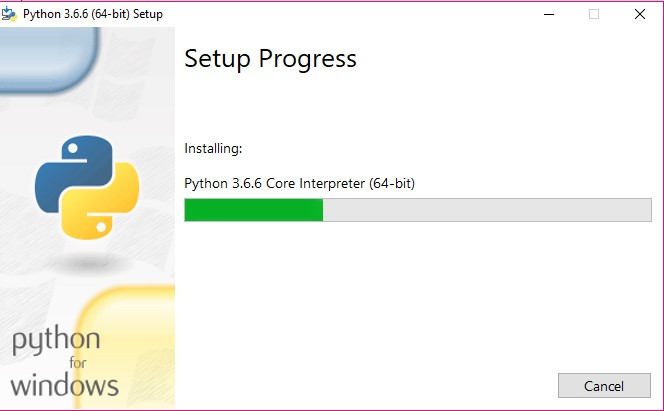
\includegraphics[width=0.75\textwidth]{pictures/python.jpg}
\caption{peroses instalasi \textit{python}}
\label{labelgambar1}
\end{figure}

\item Untuk mengecek apakan python sudah terinstall atau belum bisa menggunakan command prompt pada computer anda.
\end{enumerate}
\begin{figure}[htbp]
\centering
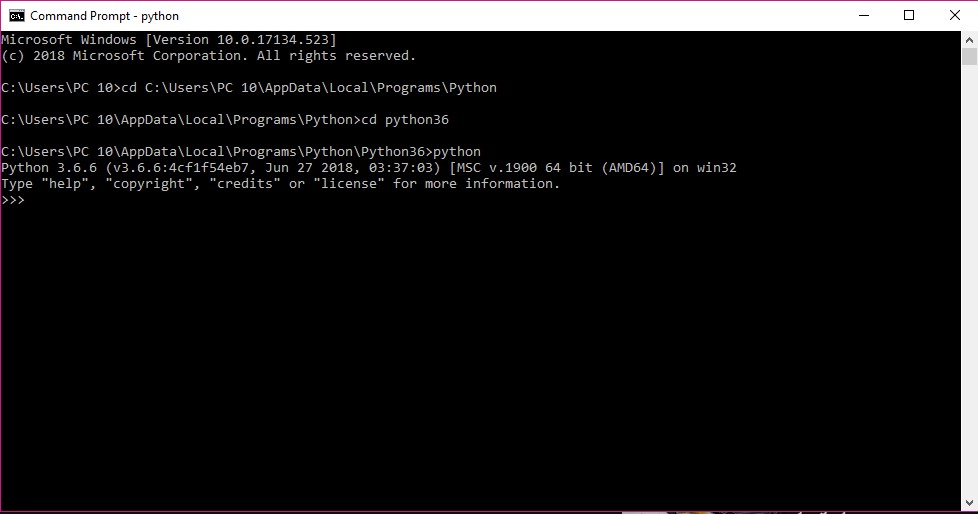
\includegraphics[width=0.75\textwidth]{pictures/pengecekanpython.jpg}
\caption{pengecekan \textit{python}}
\label{labelgambar2}
\end{figure}

